%!TEX TS-program = xelatex
\documentclass[11pt]{article}

\usepackage[english]{babel}

\usepackage{amsmath,amssymb,amsfonts}
\usepackage[utf8]{inputenc}
\usepackage[T1]{fontenc}
\usepackage{stix2}
\usepackage[scaled]{helvet}
\usepackage[scaled]{inconsolata}

\usepackage{lastpage}

\usepackage{setspace}

\usepackage{ccicons}

\usepackage[hang,flushmargin]{footmisc}

\usepackage{geometry}

\setlength{\parindent}{0pt}
\setlength{\parskip}{6pt plus 2pt minus 1pt}

\usepackage{fancyhdr}
\renewcommand{\headrulewidth}{0pt}\providecommand{\tightlist}{%
  \setlength{\itemsep}{0pt}\setlength{\parskip}{0pt}}

\makeatletter
\newcounter{tableno}
\newenvironment{tablenos:no-prefix-table-caption}{
  \caption@ifcompatibility{}{
    \let\oldthetable\thetable
    \let\oldtheHtable\theHtable
    \renewcommand{\thetable}{tableno:\thetableno}
    \renewcommand{\theHtable}{tableno:\thetableno}
    \stepcounter{tableno}
    \captionsetup{labelformat=empty}
  }
}{
  \caption@ifcompatibility{}{
    \captionsetup{labelformat=default}
    \let\thetable\oldthetable
    \let\theHtable\oldtheHtable
    \addtocounter{table}{-1}
  }
}
\makeatother

\usepackage{array}
\newcommand{\PreserveBackslash}[1]{\let\temp=\\#1\let\\=\temp}
\let\PBS=\PreserveBackslash

\usepackage[breaklinks=true]{hyperref}
\hypersetup{colorlinks,%
citecolor=blue,%
filecolor=blue,%
linkcolor=blue,%
urlcolor=blue}
\usepackage{url}

\usepackage{caption}
\setcounter{secnumdepth}{0}
\usepackage{cleveref}

\usepackage{graphicx}
\makeatletter
\def\maxwidth{\ifdim\Gin@nat@width>\linewidth\linewidth
\else\Gin@nat@width\fi}
\makeatother
\let\Oldincludegraphics\includegraphics
\renewcommand{\includegraphics}[1]{\Oldincludegraphics[width=\maxwidth]{#1}}

\usepackage{longtable}
\usepackage{booktabs}

\usepackage{color}
\usepackage{fancyvrb}
\newcommand{\VerbBar}{|}
\newcommand{\VERB}{\Verb[commandchars=\\\{\}]}
\DefineVerbatimEnvironment{Highlighting}{Verbatim}{commandchars=\\\{\}}
% Add ',fontsize=\small' for more characters per line
\usepackage{framed}
\definecolor{shadecolor}{RGB}{248,248,248}
\newenvironment{Shaded}{\begin{snugshade}}{\end{snugshade}}
\newcommand{\KeywordTok}[1]{\textcolor[rgb]{0.13,0.29,0.53}{\textbf{#1}}}
\newcommand{\DataTypeTok}[1]{\textcolor[rgb]{0.13,0.29,0.53}{#1}}
\newcommand{\DecValTok}[1]{\textcolor[rgb]{0.00,0.00,0.81}{#1}}
\newcommand{\BaseNTok}[1]{\textcolor[rgb]{0.00,0.00,0.81}{#1}}
\newcommand{\FloatTok}[1]{\textcolor[rgb]{0.00,0.00,0.81}{#1}}
\newcommand{\ConstantTok}[1]{\textcolor[rgb]{0.00,0.00,0.00}{#1}}
\newcommand{\CharTok}[1]{\textcolor[rgb]{0.31,0.60,0.02}{#1}}
\newcommand{\SpecialCharTok}[1]{\textcolor[rgb]{0.00,0.00,0.00}{#1}}
\newcommand{\StringTok}[1]{\textcolor[rgb]{0.31,0.60,0.02}{#1}}
\newcommand{\VerbatimStringTok}[1]{\textcolor[rgb]{0.31,0.60,0.02}{#1}}
\newcommand{\SpecialStringTok}[1]{\textcolor[rgb]{0.31,0.60,0.02}{#1}}
\newcommand{\ImportTok}[1]{#1}
\newcommand{\CommentTok}[1]{\textcolor[rgb]{0.56,0.35,0.01}{\textit{#1}}}
\newcommand{\DocumentationTok}[1]{\textcolor[rgb]{0.56,0.35,0.01}{\textbf{\textit{#1}}}}
\newcommand{\AnnotationTok}[1]{\textcolor[rgb]{0.56,0.35,0.01}{\textbf{\textit{#1}}}}
\newcommand{\CommentVarTok}[1]{\textcolor[rgb]{0.56,0.35,0.01}{\textbf{\textit{#1}}}}
\newcommand{\OtherTok}[1]{\textcolor[rgb]{0.56,0.35,0.01}{#1}}
\newcommand{\FunctionTok}[1]{\textcolor[rgb]{0.00,0.00,0.00}{#1}}
\newcommand{\VariableTok}[1]{\textcolor[rgb]{0.00,0.00,0.00}{#1}}
\newcommand{\ControlFlowTok}[1]{\textcolor[rgb]{0.13,0.29,0.53}{\textbf{#1}}}
\newcommand{\OperatorTok}[1]{\textcolor[rgb]{0.81,0.36,0.00}{\textbf{#1}}}
\newcommand{\BuiltInTok}[1]{#1}
\newcommand{\ExtensionTok}[1]{#1}
\newcommand{\PreprocessorTok}[1]{\textcolor[rgb]{0.56,0.35,0.01}{\textit{#1}}}
\newcommand{\AttributeTok}[1]{\textcolor[rgb]{0.77,0.63,0.00}{#1}}
\newcommand{\RegionMarkerTok}[1]{#1}
\newcommand{\InformationTok}[1]{\textcolor[rgb]{0.56,0.35,0.01}{\textbf{\textit{#1}}}}
\newcommand{\WarningTok}[1]{\textcolor[rgb]{0.56,0.35,0.01}{\textbf{\textit{#1}}}}
\newcommand{\AlertTok}[1]{\textcolor[rgb]{0.94,0.16,0.16}{#1}}
\newcommand{\ErrorTok}[1]{\textcolor[rgb]{0.64,0.00,0.00}{\textbf{#1}}}
\newcommand{\NormalTok}[1]{#1}

\newlength{\cslhangindent}
\setlength{\cslhangindent}{1.5em}
\newlength{\csllabelwidth}
\setlength{\csllabelwidth}{3em}
\newenvironment{CSLReferences}[3] % #1 hanging-ident, #2 entry spacing
 {% don't indent paragraphs
  \setlength{\parindent}{0pt}
  % turn on hanging indent if param 1 is 1
  \ifodd #1 \everypar{\setlength{\hangindent}{\cslhangindent}}\ignorespaces\fi
  % set entry spacing
  \ifnum #2 > 0
  \setlength{\parskip}{#2\baselineskip}
  \fi
 }%
 {}
\usepackage{calc} % for \widthof, \maxof
\newcommand{\CSLBlock}[1]{#1\hfill\break}
\newcommand{\CSLLeftMargin}[1]{\parbox[t]{\maxof{\widthof{#1}}{\csllabelwidth}}{#1}}
\newcommand{\CSLRightInline}[1]{\parbox[t]{\linewidth}{#1}}
\newcommand{\CSLIndent}[1]{\hspace{\cslhangindent}#1}\geometry{verbose,letterpaper,tmargin=2.2cm,bmargin=2.2cm,lmargin=2.2cm,rmargin=2.2cm}

\usepackage{lineno}
\usepackage[nolists,noheads]{endfloat}

\pagestyle{plain}

\tolerance=1
\emergencystretch=\maxdimen
\hyphenpenalty=10000
\hbadness=10000

\doublespacing

\fancypagestyle{normal}
{
  \fancyhf{}
  \fancyfoot[R]{\footnotesize\sffamily\thepage\ of \pageref*{LastPage}}
}
\begin{document}
\raggedright
\thispagestyle{empty}
{\Large\bfseries\sffamily Thesis proposal}
\vskip 5em

%
\href{https://orcid.org/0000-0002-6506-6487}{Michael D.\,Catchen}%
%
\,\textsuperscript{1,2}

\textsuperscript{1}\,McGill University\quad \textsuperscript{2}\,Québec
Centre for Biodiversity Sciences


\textbf{Correspondance to:}\\
Michael D. Catchen --- \texttt{michael.catchen@mail.mcgill.ca}\\

\vfill
This work is released by its authors under a CC-BY 4.0 license\hfill\ccby\\
Last revision: \emph{\today}

\clearpage
\thispagestyle{empty}

\vfill
The proposal for my thesis, \emph{Simulation models for predictive
ecology}



\vfill

\clearpage
\linenumbers
\pagestyle{normal}

\hypertarget{introduction}{%
\section{Introduction}\label{introduction}}

\textbf{P1}

Within the last several hundred years, human activity has rapidly
changed Earth's atmosphere, oceans, and surface. Greenhouse gas
emissions have caused an increase the temperature of both Earth's
terrestial surface and its oceans, and both agricultural and urban
development has rapidly reshaped the cover of Earth's surface. These the
bulk of this change has occurred within the last several hundred years,
a geological instant, potentially inducing shocks to ecosystems that
could threated their integrity (\textbf{Scheffer?}). As a result
understanding and predicting how ecosystems will change in the future,
\emph{ecological forecasting}, and making making descisions based on
these predictions mitigating the consequences of this change, on
ecosystems has emerged as an imperative for ecology and environmental
science {[}Dietze (2017);{]}.

\textbf{P2}

However, robust forecasting of ecological processes will change in the
future is, to say the least, quite difficult (Beckage \emph{et al.}
2011; Petchey \emph{et al.} 2015). This difficultly is compounded by a
few factors, the first being that sampling ecosystems is not easy.
Ecological data is often biased, and noisey, spatially and temporally
sparse. As a result \emph{ecosystem monitoring} (Makiola \emph{et al.}
2020) has emerged as an imperative. Developing a system for ecological
observation, which is able to coordinate across locations.
(\textbf{AndyUrbanBiomonitoring?} paper).

The second major challenge in forecasting ecosystems is that the
underlying dynamics of most ecological processes are fundementally
unknown (and unknowable) and instead must be inferred.

Much of the history of quantitatively modeling ecosystems have been done
in the language of dynamical systems, describing how the value of an
observable state of the system, represented by a vector of numbers
\([x_1, x_2, \dots, x_n]^T = \vec{x}\) changes as over time. It turns
out to be much more effective to, rather than attempt to directly model
\(\vec{x}(t)\) itself, to instead describe how \(\vec{x}\) changes from
one timestep to the next, yielding models in the form of differential
equations in continuous-time settings--\(\frac{dx}{dt} = f(x)\)-- or
difference equations in discrete-time
settings--\(x_t = f(x_{t-1})\)--where
\(f:\mathbb{R}^n \to \mathbb{R}^n\) is an arbitrary function describing
how the system changes on a moment-to-moment basis (e.g.~in the context
of communities, \(f\) could be Lotka-Voltera, Holling-Type-III or
DeAngelis-Beddington functional response). The form of this functional
response in real systems is effectively unknown, and some forms are
inherently more ``forecastable'' than others (Chen \emph{et al.} 2019).

\textbf{P3}

However, we run into many problems when aiming to apply this type of
model to empirical data in ecology.

The initial success of ODE models can be traced back to the larger
program of ontological reductionism, which became the de facto apporoach
model physical sciences after its early success in physics, which, by
the time ecology was becoming a quantitative science (sometime in the
20th century, depending on who you ask), became the foundation for early
quantitative models in ecology.

But ecosystems are perhaps the quintessential example of system that
cannot be understood simply by iterative reduction of its components.
Emergent phenomena, mechanisms at different scales, etc.

Some have been explored in the ecological literature: (1) Some
applications of dynamic models in ecology assume long-run equilibrium.
(2) Stochasticity

\begin{enumerate}
\def\labelenumi{(\arabic{enumi})}
\setcounter{enumi}{2}
\tightlist
\item
  Ecological processes vary across more variables than the tools of
  analytic models are suited for. As the number of variables in an
  analytic model increases, so does the ability of the scientist to
  decern clear relationships between them, and so does overfitting
  potential. Curse of dimensionality--- Until the 20th century, no
  theory of the gravitational dynamics of more than 2 bodies.
  Understanding the gravitational dynamics of more than two planets with
  any reliability proved difficult. Using the same models (diffeqs), how
  could we adequately predict ecosystems?
\end{enumerate}

\textbf{P4}

The term \emph{ecological forecasting} implicitly creates an analogy
between predicting how ecosystems will change in the future by using the
term ``forecasting''---the most immediate analog being the success story
of weather forecasting via numerical weather prediction (NWP).

Although it is become almost hack to complain about the dang weather
forecast being wrong, over the least 50 years the (Bauer \emph{et al.}
2015).

The success of NWP, and the Earth observations that support it should
serve as a template for development of a system for monitoring Earth's
biodiversity. Much like ecology, NWP is faced with high-dimensional
systems that are governed by different mechanisms at different scales.

NWP has worked because it incorporates information about data and
meteorological processes collected at difference scales into models
that. Use of computational methods in NWP.

Much as one would not aim to forecast the weather in Quebec by applying
Navier-Stokes, forecasting ecological systems must

Transition to simulation as the solution: shift toward approach of
building models that \emph{generate} data.

(resolving the semantic ambuity of what differentiates ``mechanistic''
vs ``phenomological'' models is out of scope for now).

More broadly a reflection reflect ecology lagging behind the statistical
methods used in sciences that face similar challenges (many dimensions,
many mechanisms at different scales, each with stochasticity). Chaotic
dynamics emerge from simple analytic models, and . Whether ecosystems
actually exhibit chaotic behavior is a different question.

\textbf{P5}

But forecasting isn't the only difficult problem here.

Transition to theme of optimization given unknown information. A
forecast gives us a range of future values with uncertainty around them.
Further a convenient property that a forecasting model's uncertainty
goes up over time (if we assume the underlying process is Markov--this
is a strong assumption but oft true of the models we fit to temporal
data)

In face of uncertainty, decision making is an optimization problem. We
have some goal state for the future, and some estimate of what the state
of the world will be given a set of actions. Frame optimization problem
mathematically an introduce concept of solution-space and constraint.

Indeed Marx's most well known quote that ``philosophers have hitherto
only interpreted the world in various ways; the point is to change it.''
and a necessary step toward establishing a just and sustainable world.

\begin{figure}
\hypertarget{fig:thesis}{%
\centering
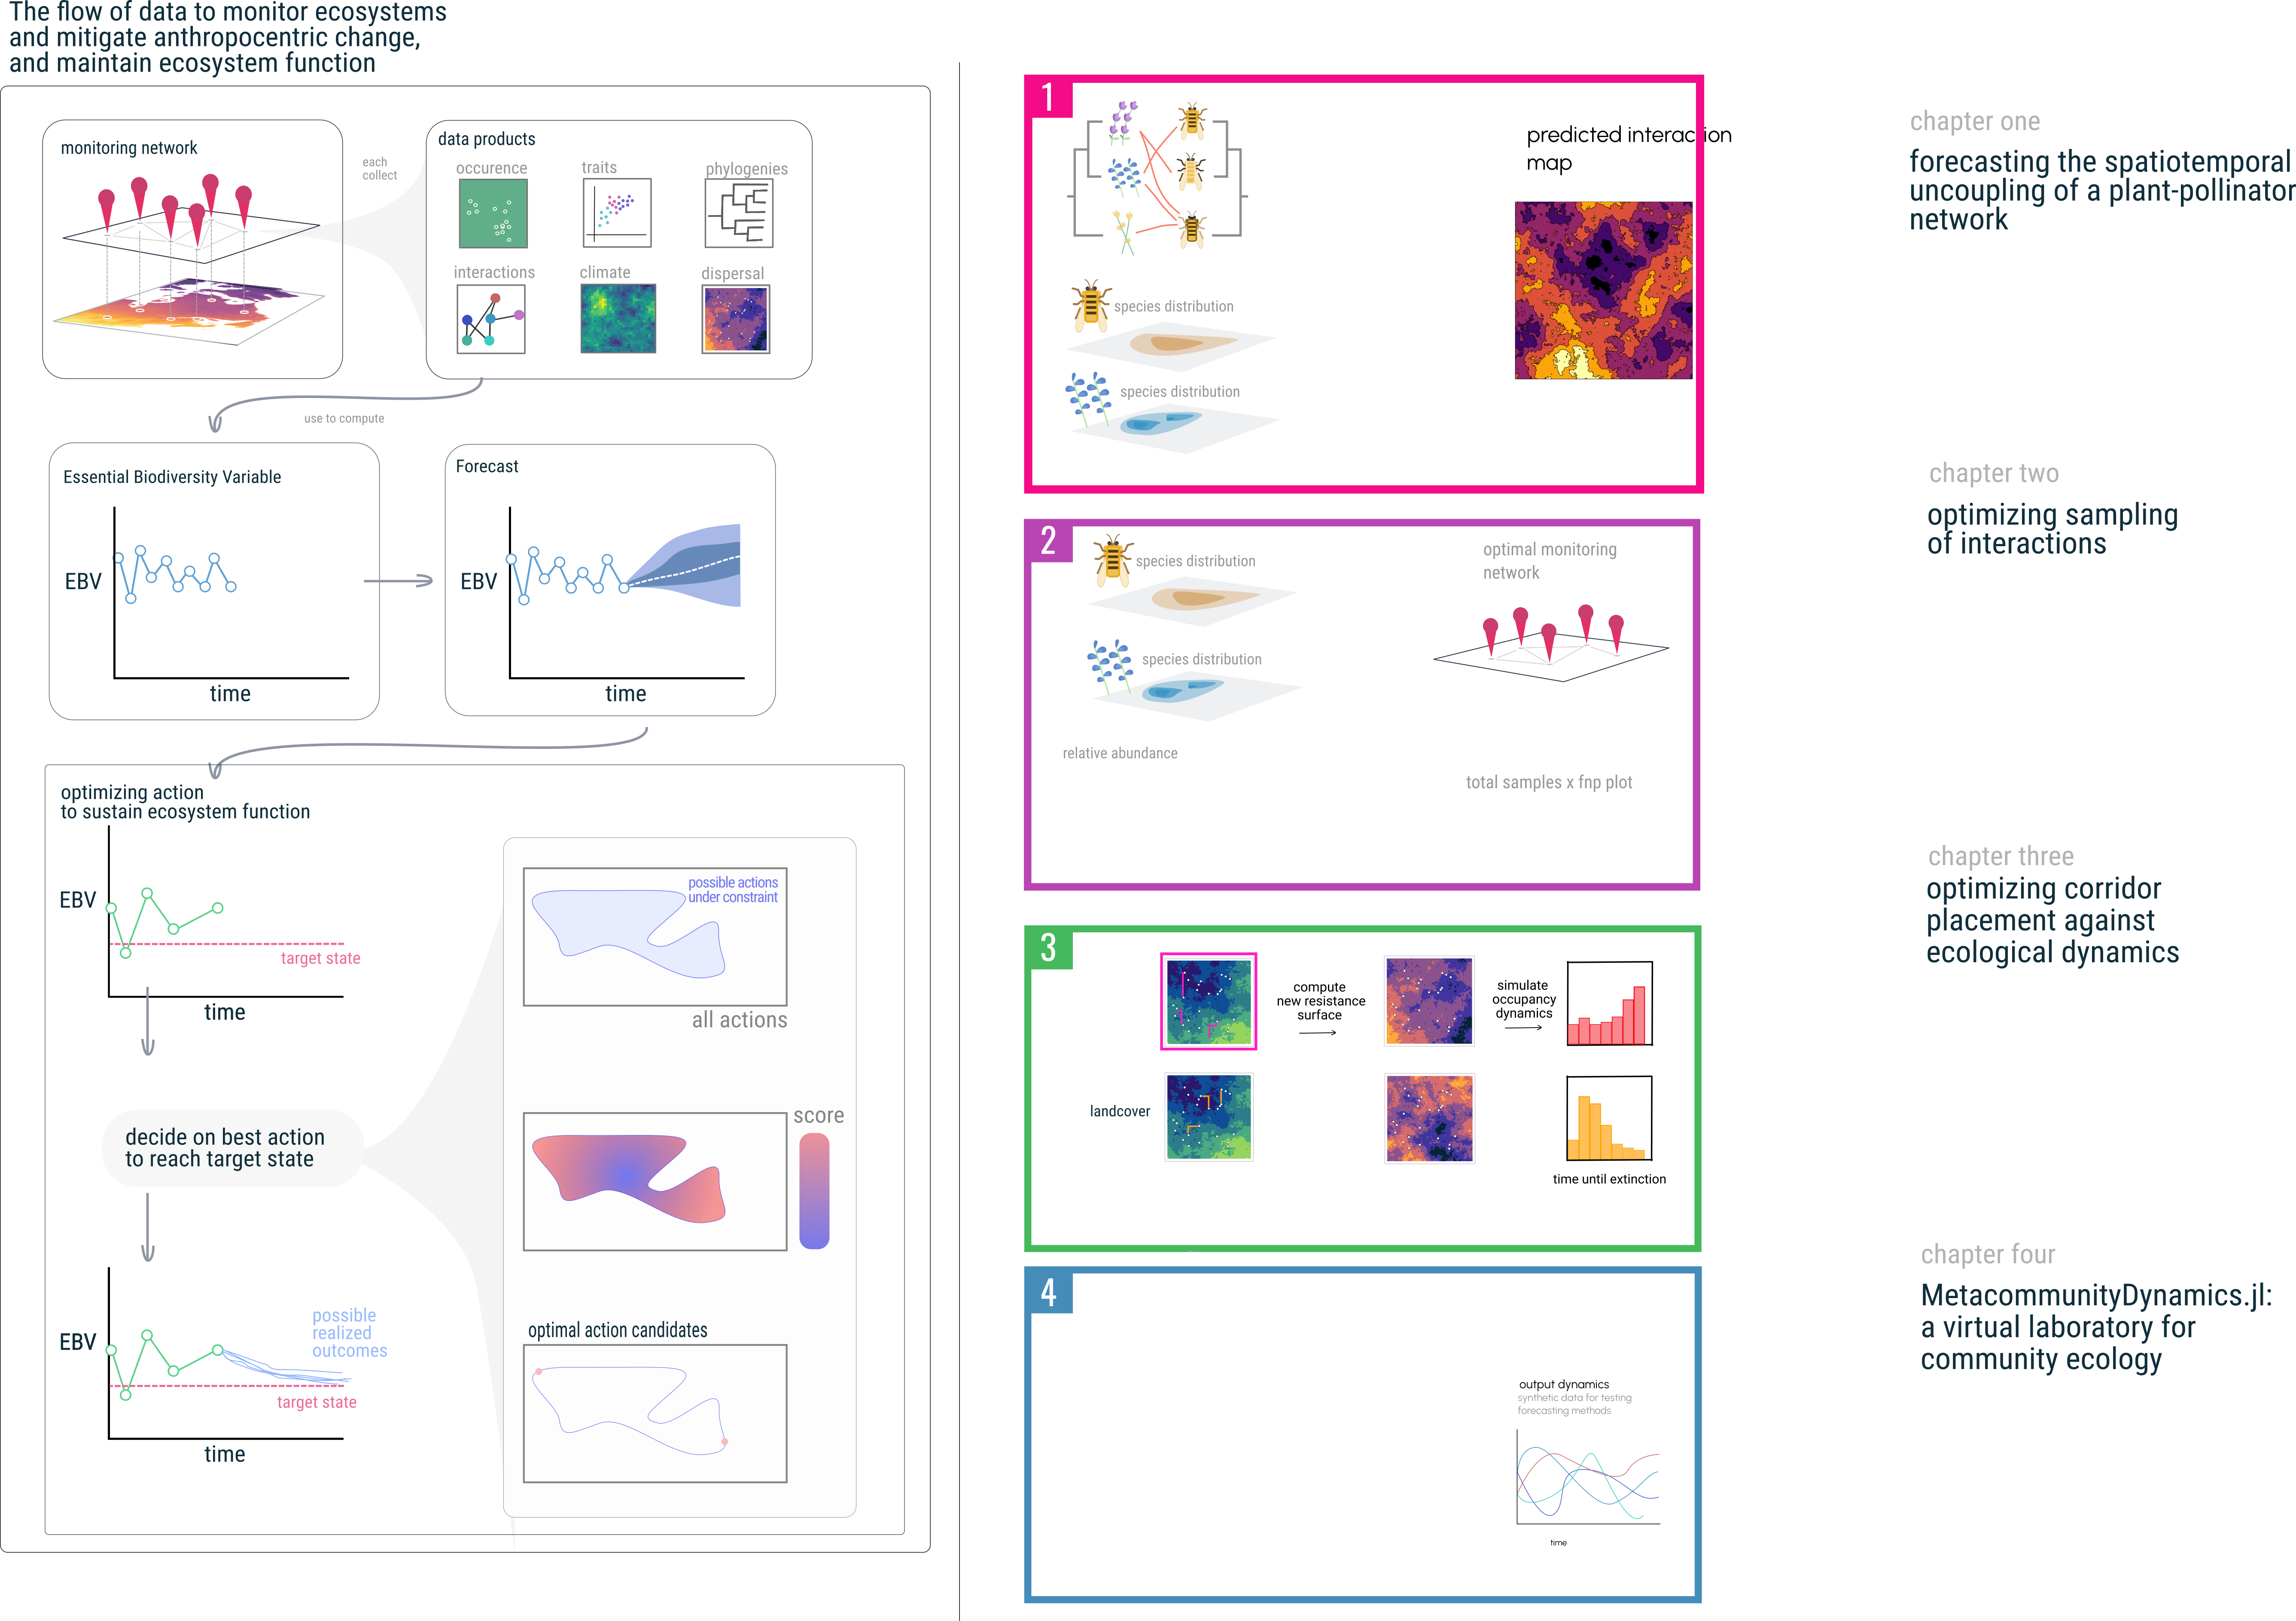
\includegraphics{./figures/thesisconcept.png}
\caption{thesis concept}\label{fig:thesis}
}
\end{figure}

\textbf{P6 -- final intro para}

Three major components here: 1) Ecosystem monitoring, 2) Forecasting
using the products of that monitoring, and 3) Choosing the best possible
mitigation strategy.

This flow is outlined in the left panel of fig.~\ref{fig:thesis}

\hypertarget{chapter-one-forecasting-the-spatial-uncoupling-of-a-plant-pollinator-network}{%
\section{Chapter One: Forecasting the spatial uncoupling of a
plant-pollinator
network}\label{chapter-one-forecasting-the-spatial-uncoupling-of-a-plant-pollinator-network}}

Plants and pollinators form interaction networks, called the
``architecture of biodiversity'' (\textbf{Jordano2007?}).

The stability, function, and persistance of ecosystems relies on the
structure of these interactions. Antropogenic change threatens to
unravel these networks. Two aspects to this change: spatial and
temporal. Spatially, range shifts along elevational gradient, and
temporall, phenological shifts.

The issue is that we don't really know what interactions are like now.
So not only do we need to predict with data that is spatially and
temporally sparse and likely to contain many interaction
``false-negatives'' (\textbf{Strydom2021?})

This chapter uses several years of data on bee-flower phenology and
interactions, combined with spatial records of species occurrence via
GBIF, to forecast how much overlap there will be between
plants/pollinators in space/time.

In stages, (1) take data from multiple sites to predict a spatial
metaweb of \emph{Bombus}-flower interactions across Colorado. (2)
Predict how these spatial distributions will change under CMIP6. and (3)
quantify the lack of overlap between species for which there is a
predicted

\textbf{CH1 concept figure}

\hypertarget{data}{%
\subsection{Data}\label{data}}

The data for this chapter is derived from multiple souces and can be
split into three categories. (1) Field data from three different
locations acvross Colorado. All field sites have multiple plots across
an elevational gradient.

System description: lots of data on \emph{Bombus} (bumblebees) and
wildflowers. Three different sites, (7/7/3) years each, each covering an
elevational gradient.

\hypertarget{methods}{%
\subsection{Methods}\label{methods}}

Split the process into parts.

\begin{enumerate}
\def\labelenumi{\arabic{enumi})}
\tightlist
\item
  Building an interaction prediction model. 2) Make it spatial based on
  distributions. 3) Forecast distributions based on CMIP6.
\end{enumerate}

\hypertarget{preliminary-results}{%
\subsection{Preliminary Results}\label{preliminary-results}}

\begin{enumerate}
\def\labelenumi{\arabic{enumi})}
\tightlist
\item
  we got a tree
\end{enumerate}

Transition to next chapter by discussing uncertainty in interaction
prediction across space.

\hypertarget{chapter-two-optimizing-spatial-sampling-of-species-interactions}{%
\section{Chapter Two: Optimizing spatial sampling of species
interactions}\label{chapter-two-optimizing-spatial-sampling-of-species-interactions}}

There are false-negatives in interation data. Co-occurrence is not the
same thing as interaction (\textbf{cite?}), but often is used as a
proxy.

This chapter unravels the relationship between a given species relative
abundance and the sampling effort needed to adequately understand this
species distribution and interactions.

There is more than one way to observe a false-negative.

\begin{figure}
\centering
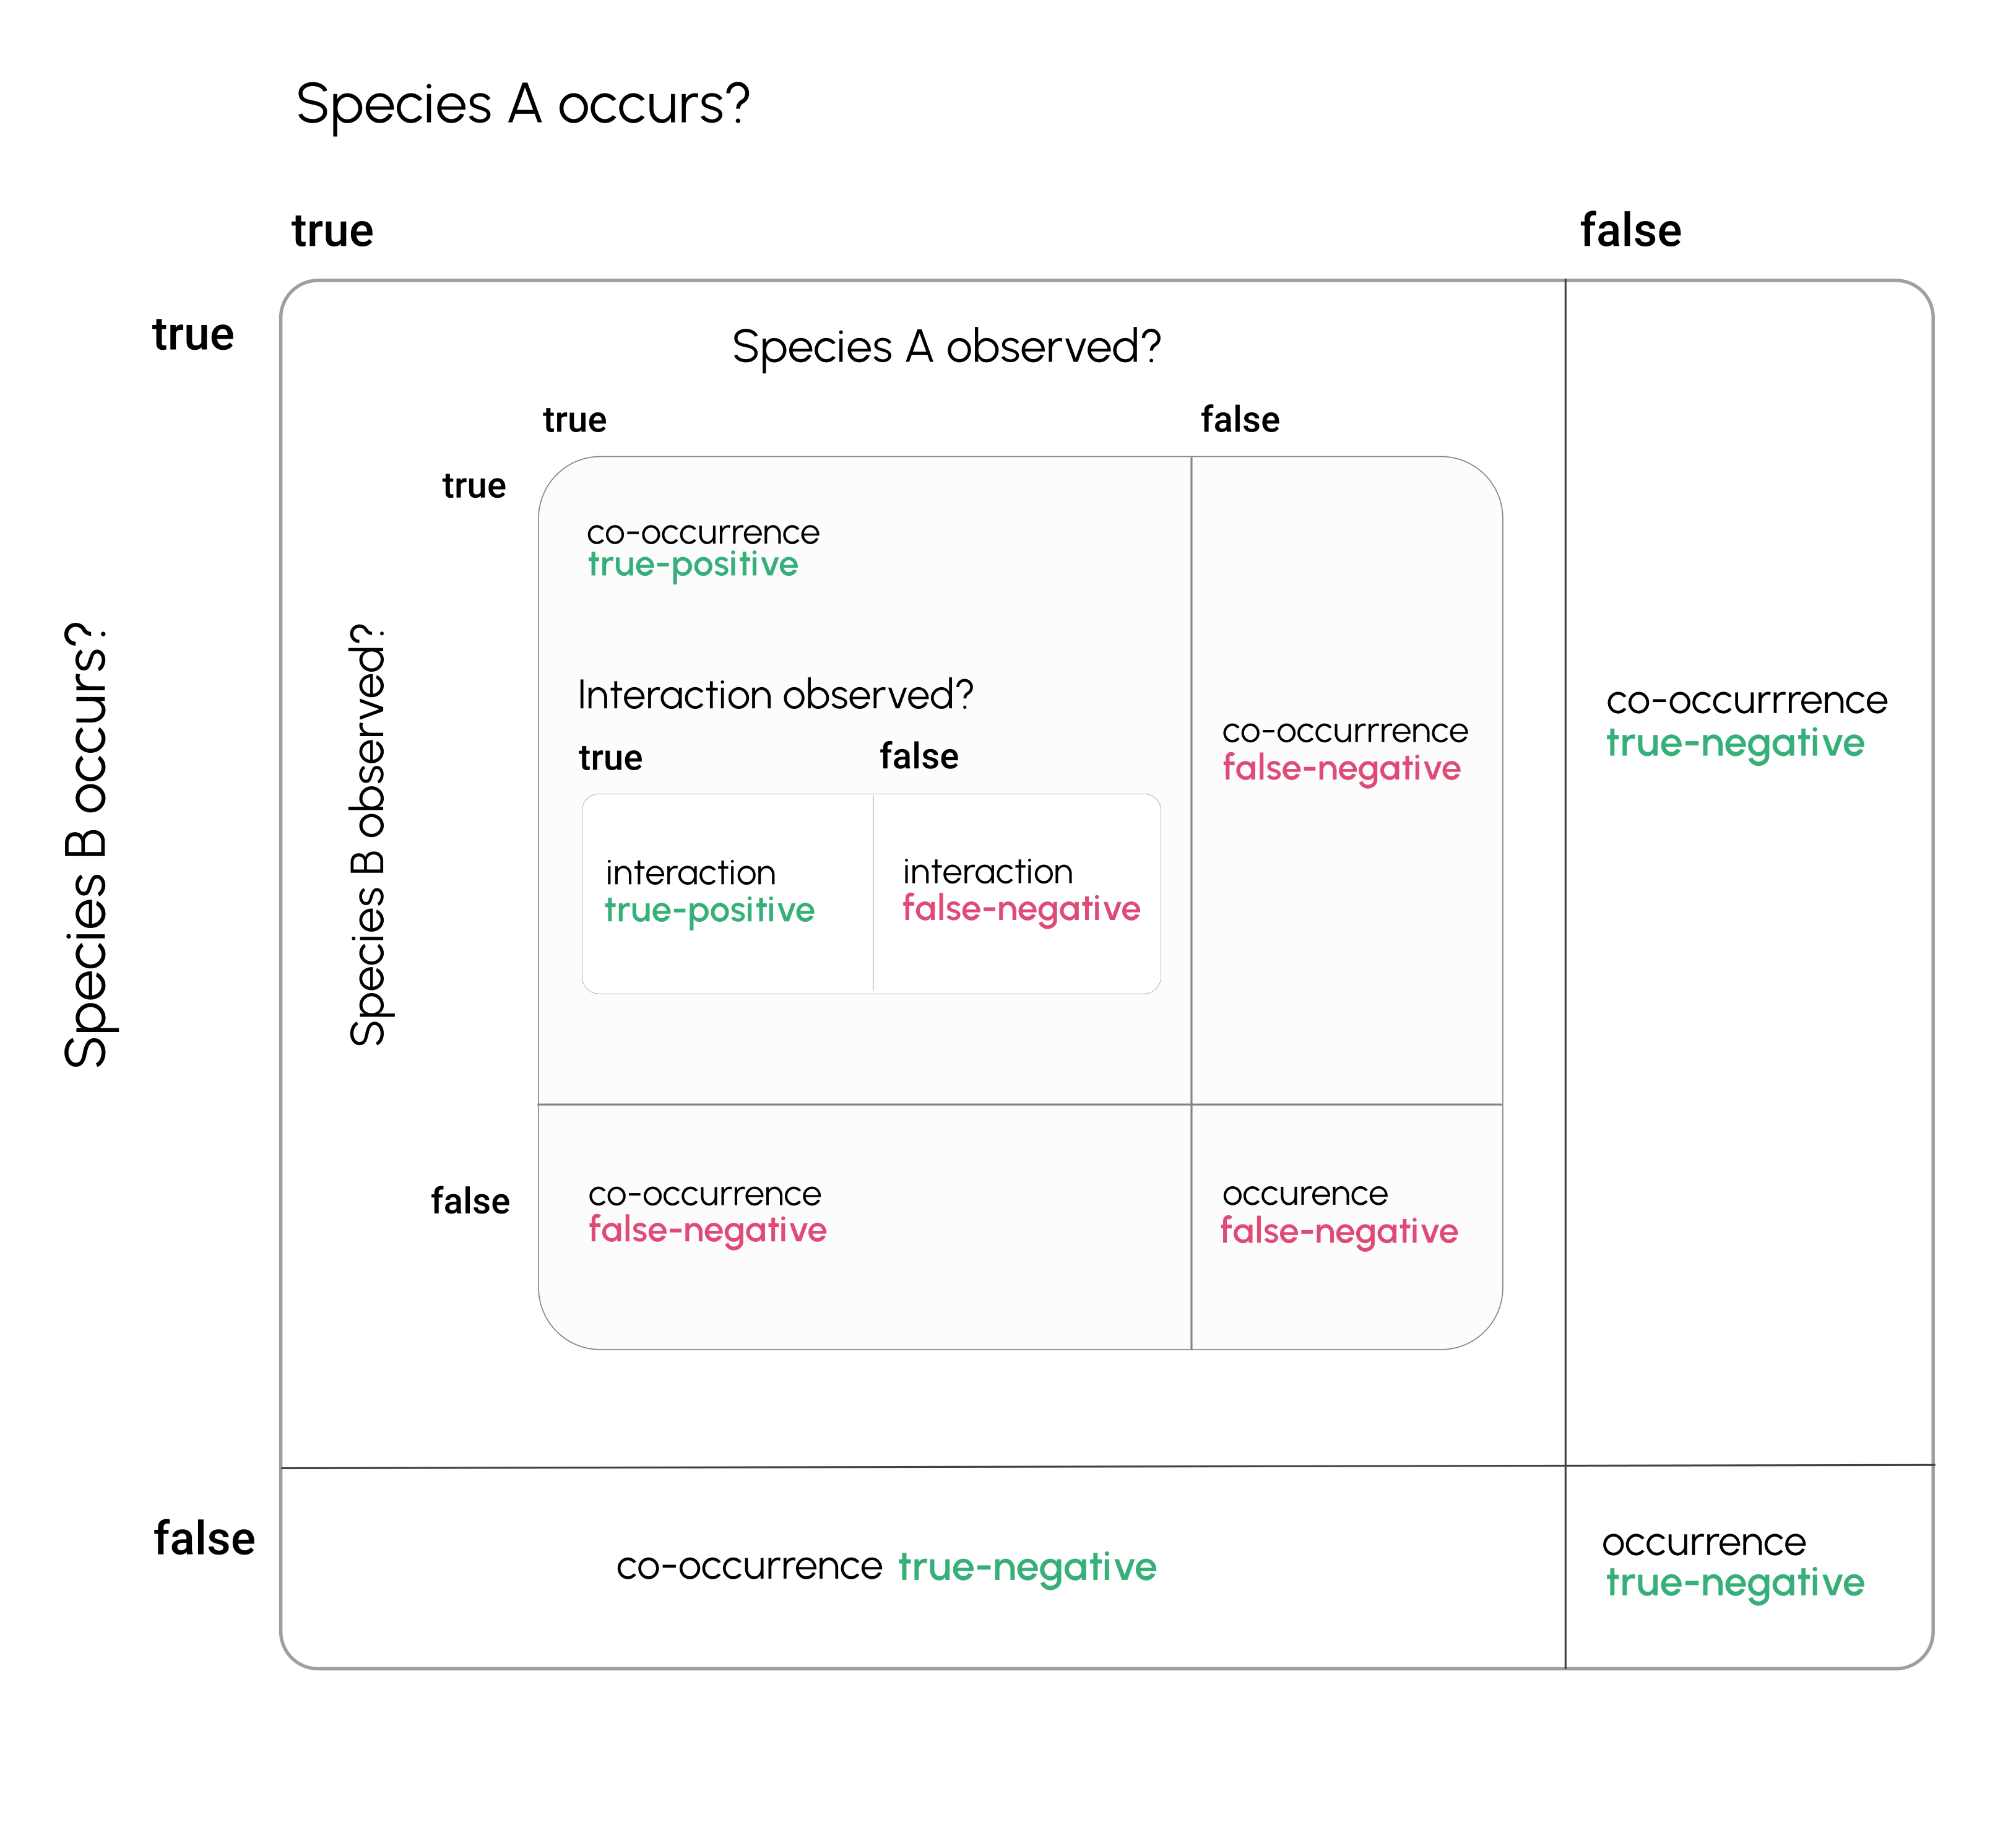
\includegraphics{./figures/ch2.png}
\caption{taxonomy of false negatives}
\end{figure}

It begins with a conceptual framework for understanding the difference
in false-negatives in occurrence, co-occurrence, and interactions
(fig.~3). We use a null model of the relative-abundance distribution
(Hubbell 2001) to simulate realized false-negatives as a function of
varying sampling effort.

This also goes on to includes testing some assumptions of the model with
empirical data fig.~\ref{fig:4}. which indicate our neutral model, if
anything, underestimates the probability of false-negatives due to
positive correlations in co-occurrence in two spatially replicated
networks (Thompson \& Townsend 2000; Hadfield \emph{et al.}
2014)---further I'm planning to add the field data from chapter one into
this anlysis once complete.

\begin{figure}
\centering
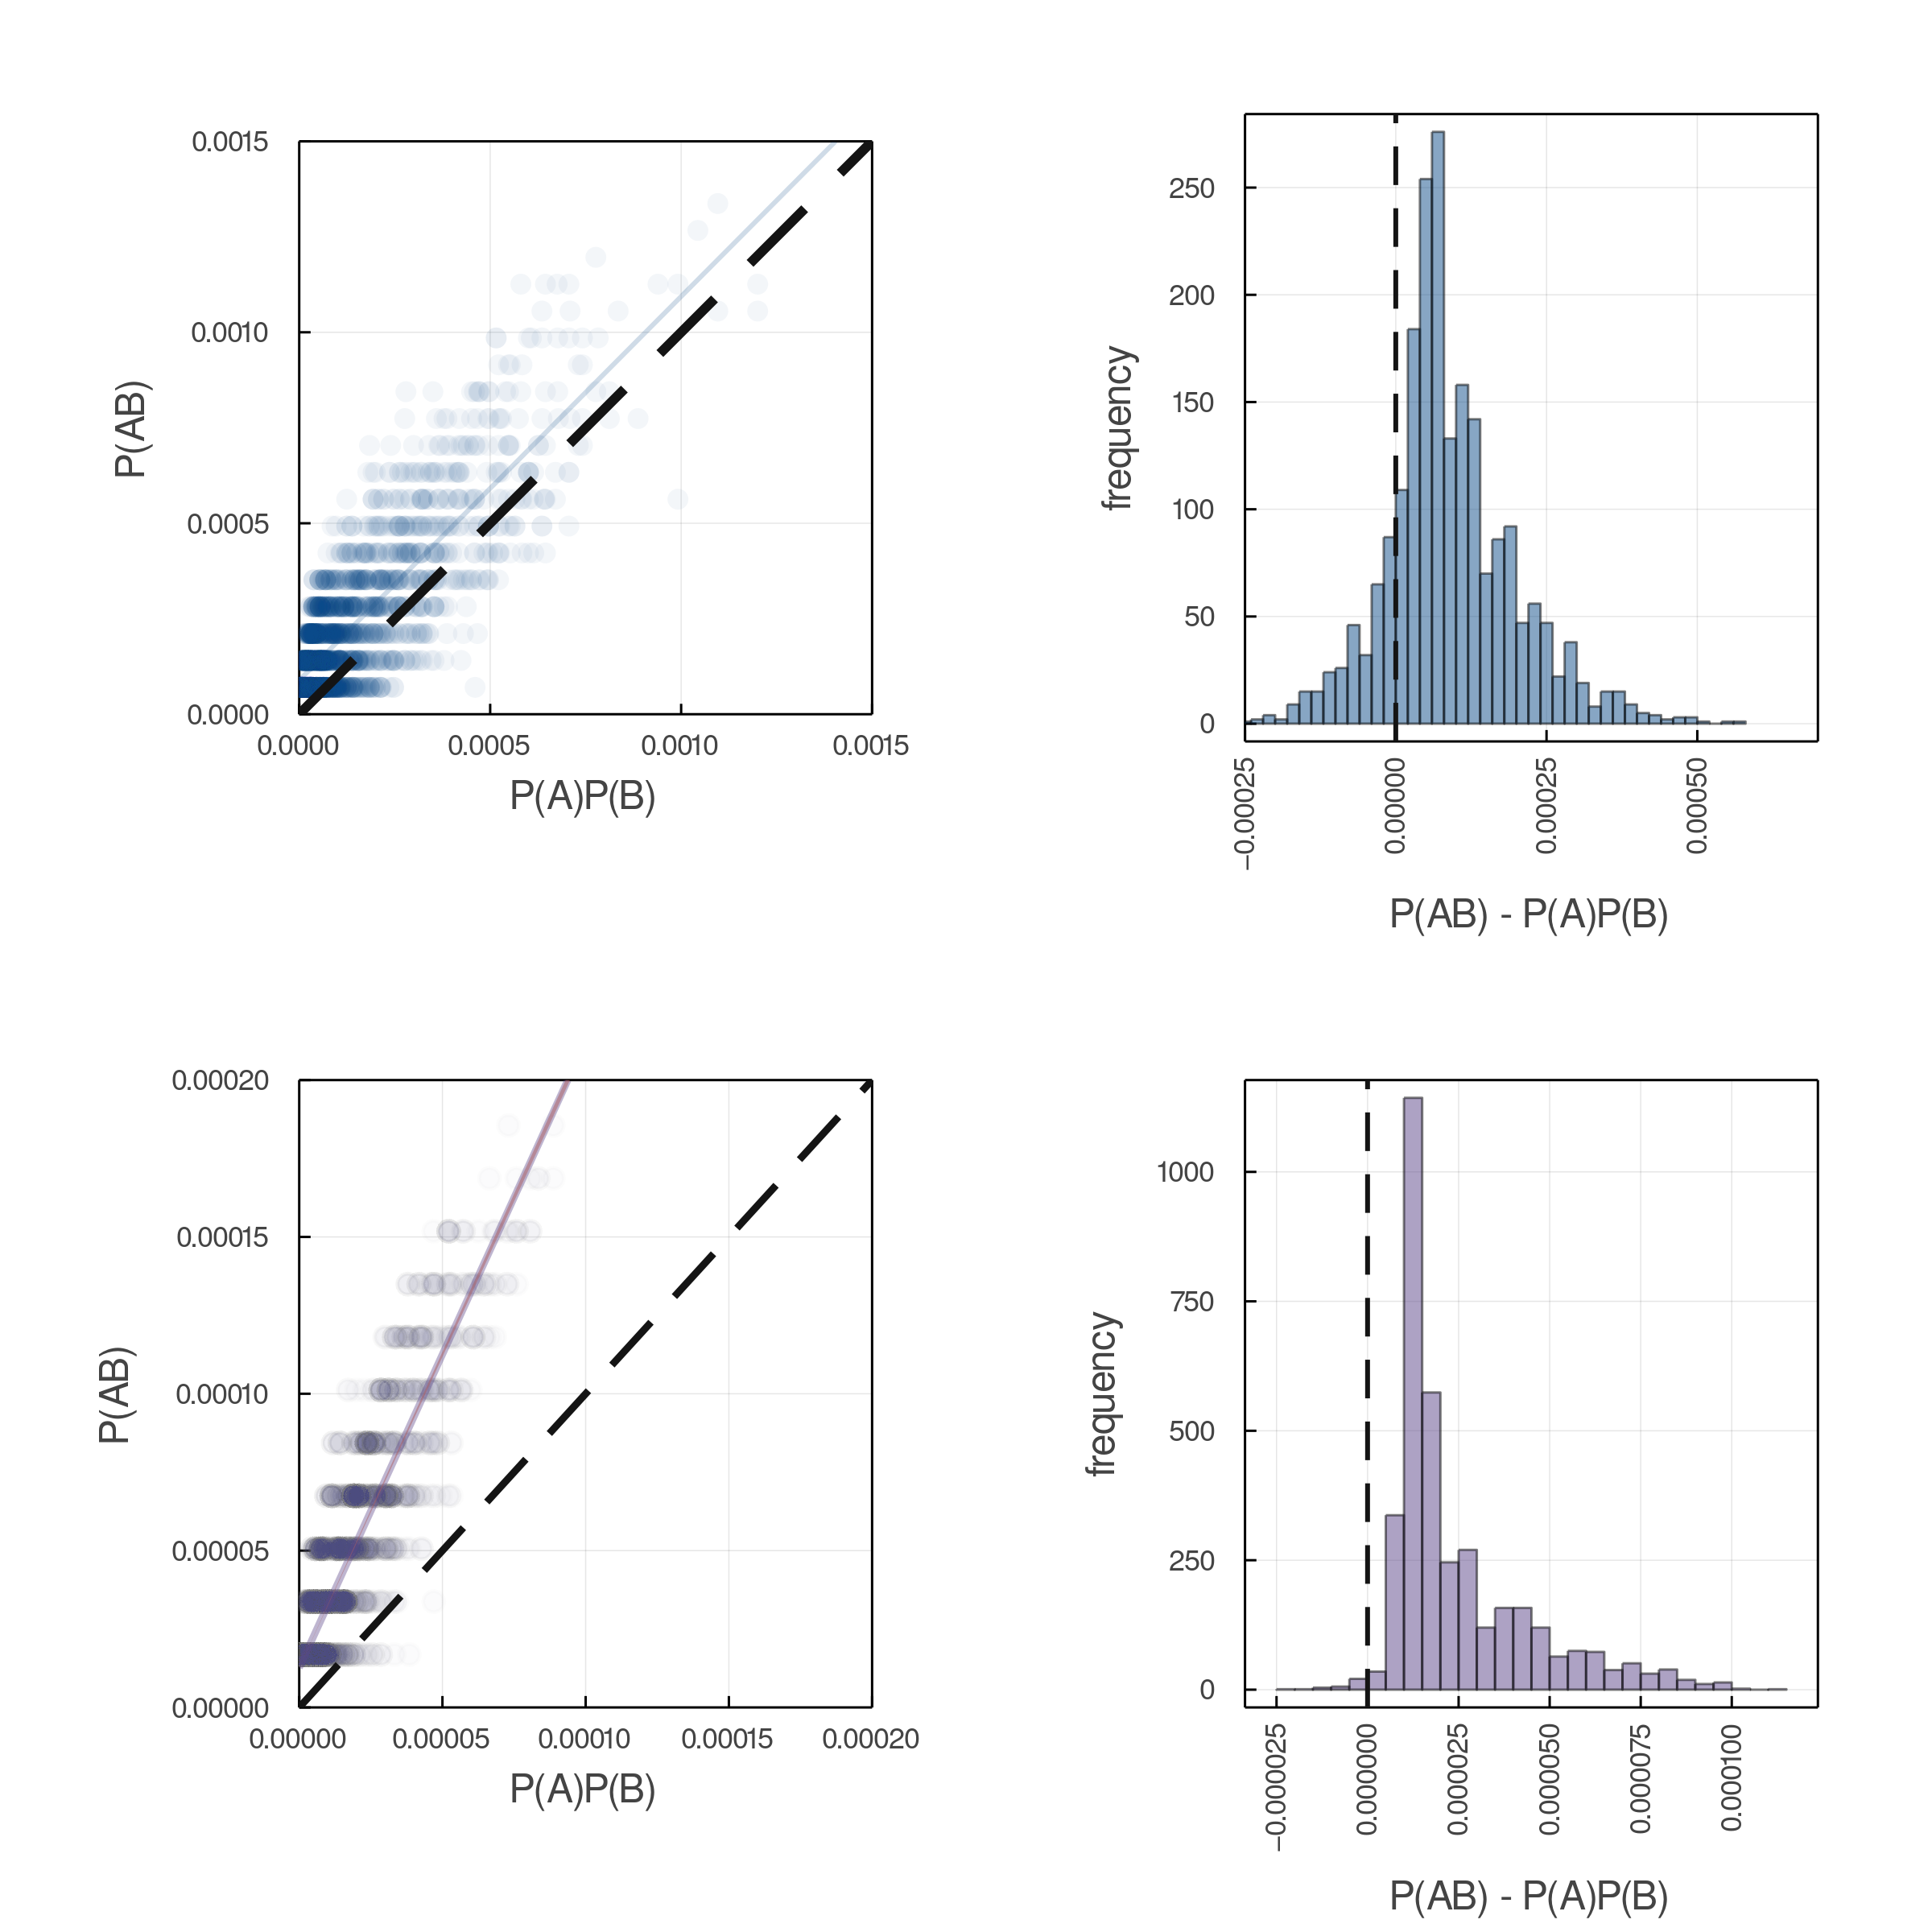
\includegraphics{./figures/positiveassociations.png}
\caption{f}
\end{figure}

new addition: - simulate species distribution and efficacy of detection
given a set of observation points where the dist from observation site
decays. optimize set of repeated sampling locations L for a \emph{known}
distribution D. address SDM not being the territory

\hypertarget{results}{%
\subsection{Results}\label{results}}

\begin{itemize}
\tightlist
\item
  nonrandom association figure sampling effort under neutral model
\end{itemize}

\hypertarget{chapter-three-optimizing-corridor-placement-against-ecological-dynamics}{%
\section{Chapter Three: Optimizing corridor placement against ecological
dynamics}\label{chapter-three-optimizing-corridor-placement-against-ecological-dynamics}}

Promoting landscape connectivity is important to mitigate the effects of
land-use change on Earth's biodiversity. However, the practical
realities of conservation mean that there is a limitation on how much we
can modify landscapes in order to do this. So what is the best place to
put a corridor given a constraint on how much surface-area you can
change in a landscape? This is the question this chapter seeks to
answer. Models for proposing corridor locations have been developed, but
are limited in that are not developed around promoting some element of
ecosystem function, but instead by trying to find the path of least
resistance given a resistance surface (Peterman 2018).

This chapter proposes a general algorithm for optimizing corridor
placement based on a measurement of ecosystem functioning derived from
simulations run on a proposed landscape modification. We propose various
landscape modifications which alter the cover of a landscape,
represented as a raster (fig.~6, left). We then compute a new resistance
surface based on the proposed landscape modification, and based on the
values of resistance to dispersal between each location we simulate
spatially-explicit metapopulation dynamics model (Hanski \& Ovaskainen
2000; Ovaskainen \emph{et al.} 2002) to estimate a distribution of time
until extinction for each landscape modification (fig.~6, right).

\hypertarget{methods-1}{%
\subsection{Methods}\label{methods-1}}

\begin{itemize}
\tightlist
\item
  land cover -\textgreater{} resistance -\textgreater{} extinction time
  simulated annealing to
\item
  optimize landscape optimization
\end{itemize}

\hypertarget{ch4-a-software-note-on-the-resulting-packages.}{%
\section{CH4 a software note on the resulting
packages.}\label{ch4-a-software-note-on-the-resulting-packages.}}

(MetacommunityDynamics.jl: a virtual laboratory for community ecology):
a collection of modules in the Julia language for different aspects of
metacommunity ecology, including most of the code used for the preceding
chapters.

\begin{figure}
\centering
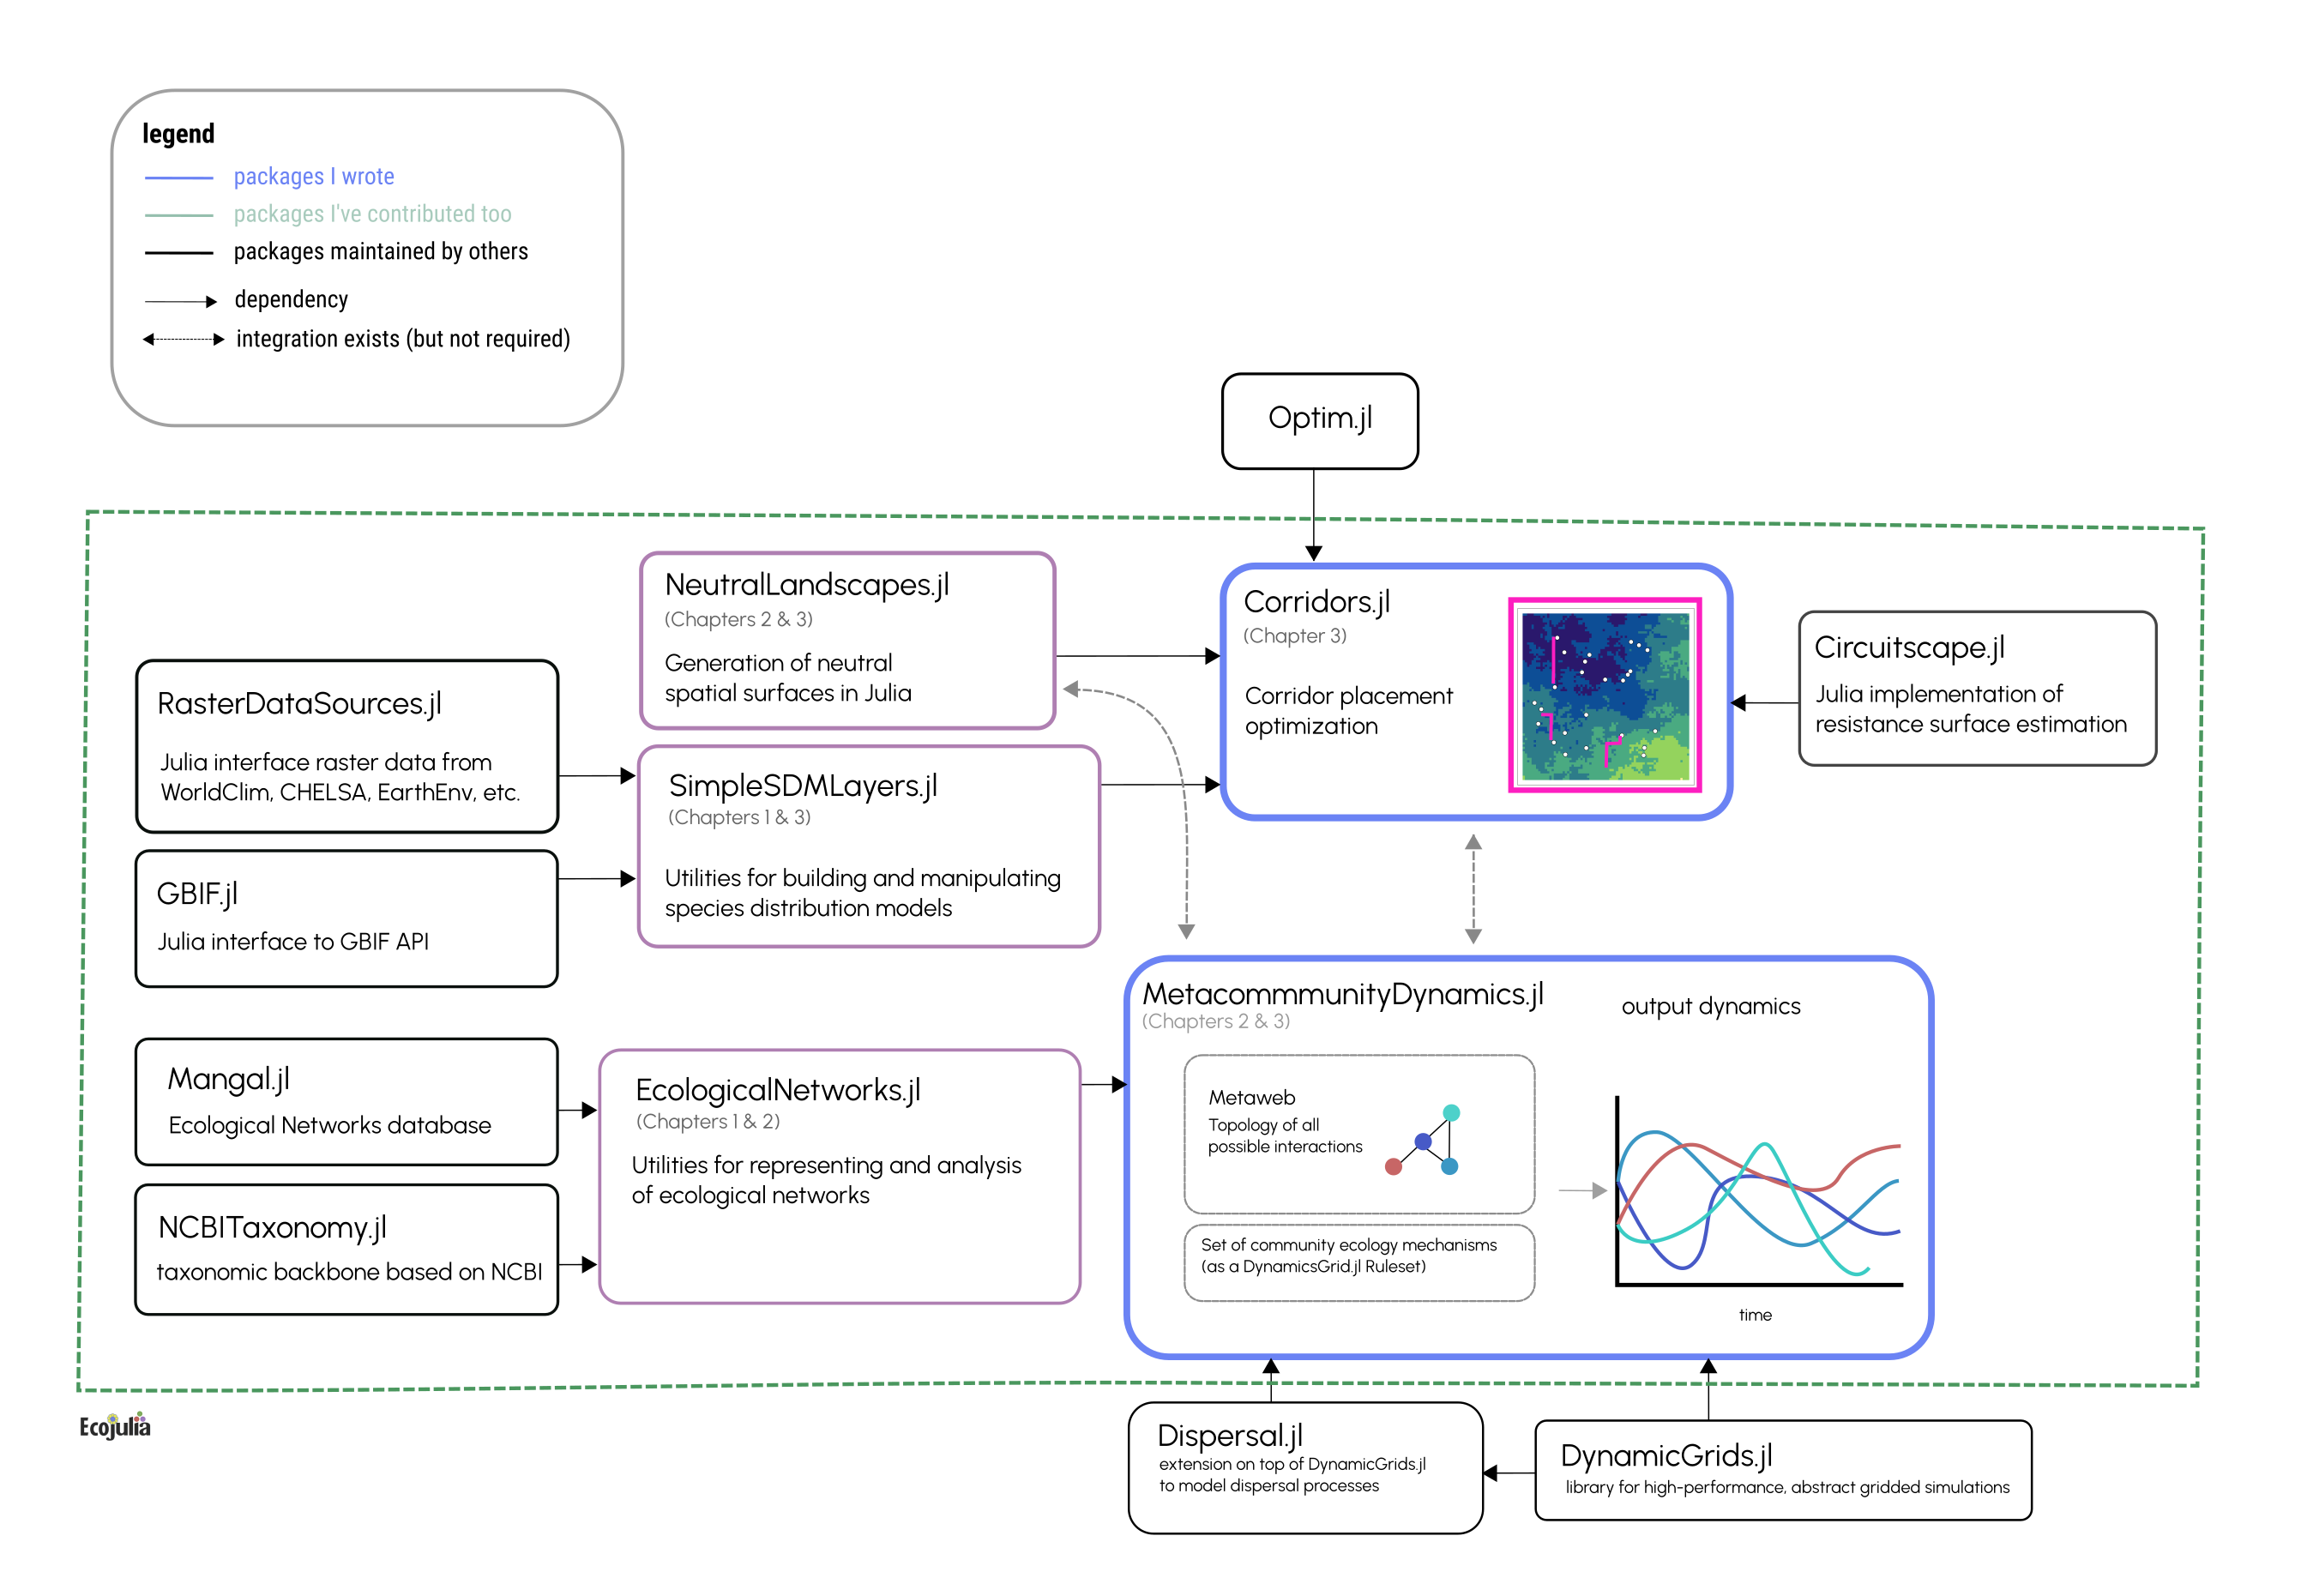
\includegraphics{./figures/software.png}
\caption{todo}
\end{figure}

\hypertarget{conclusion}{%
\section{Conclusion}\label{conclusion}}

\hypertarget{appendix}{%
\section{Appendix}\label{appendix}}

\begin{figure}
\centering
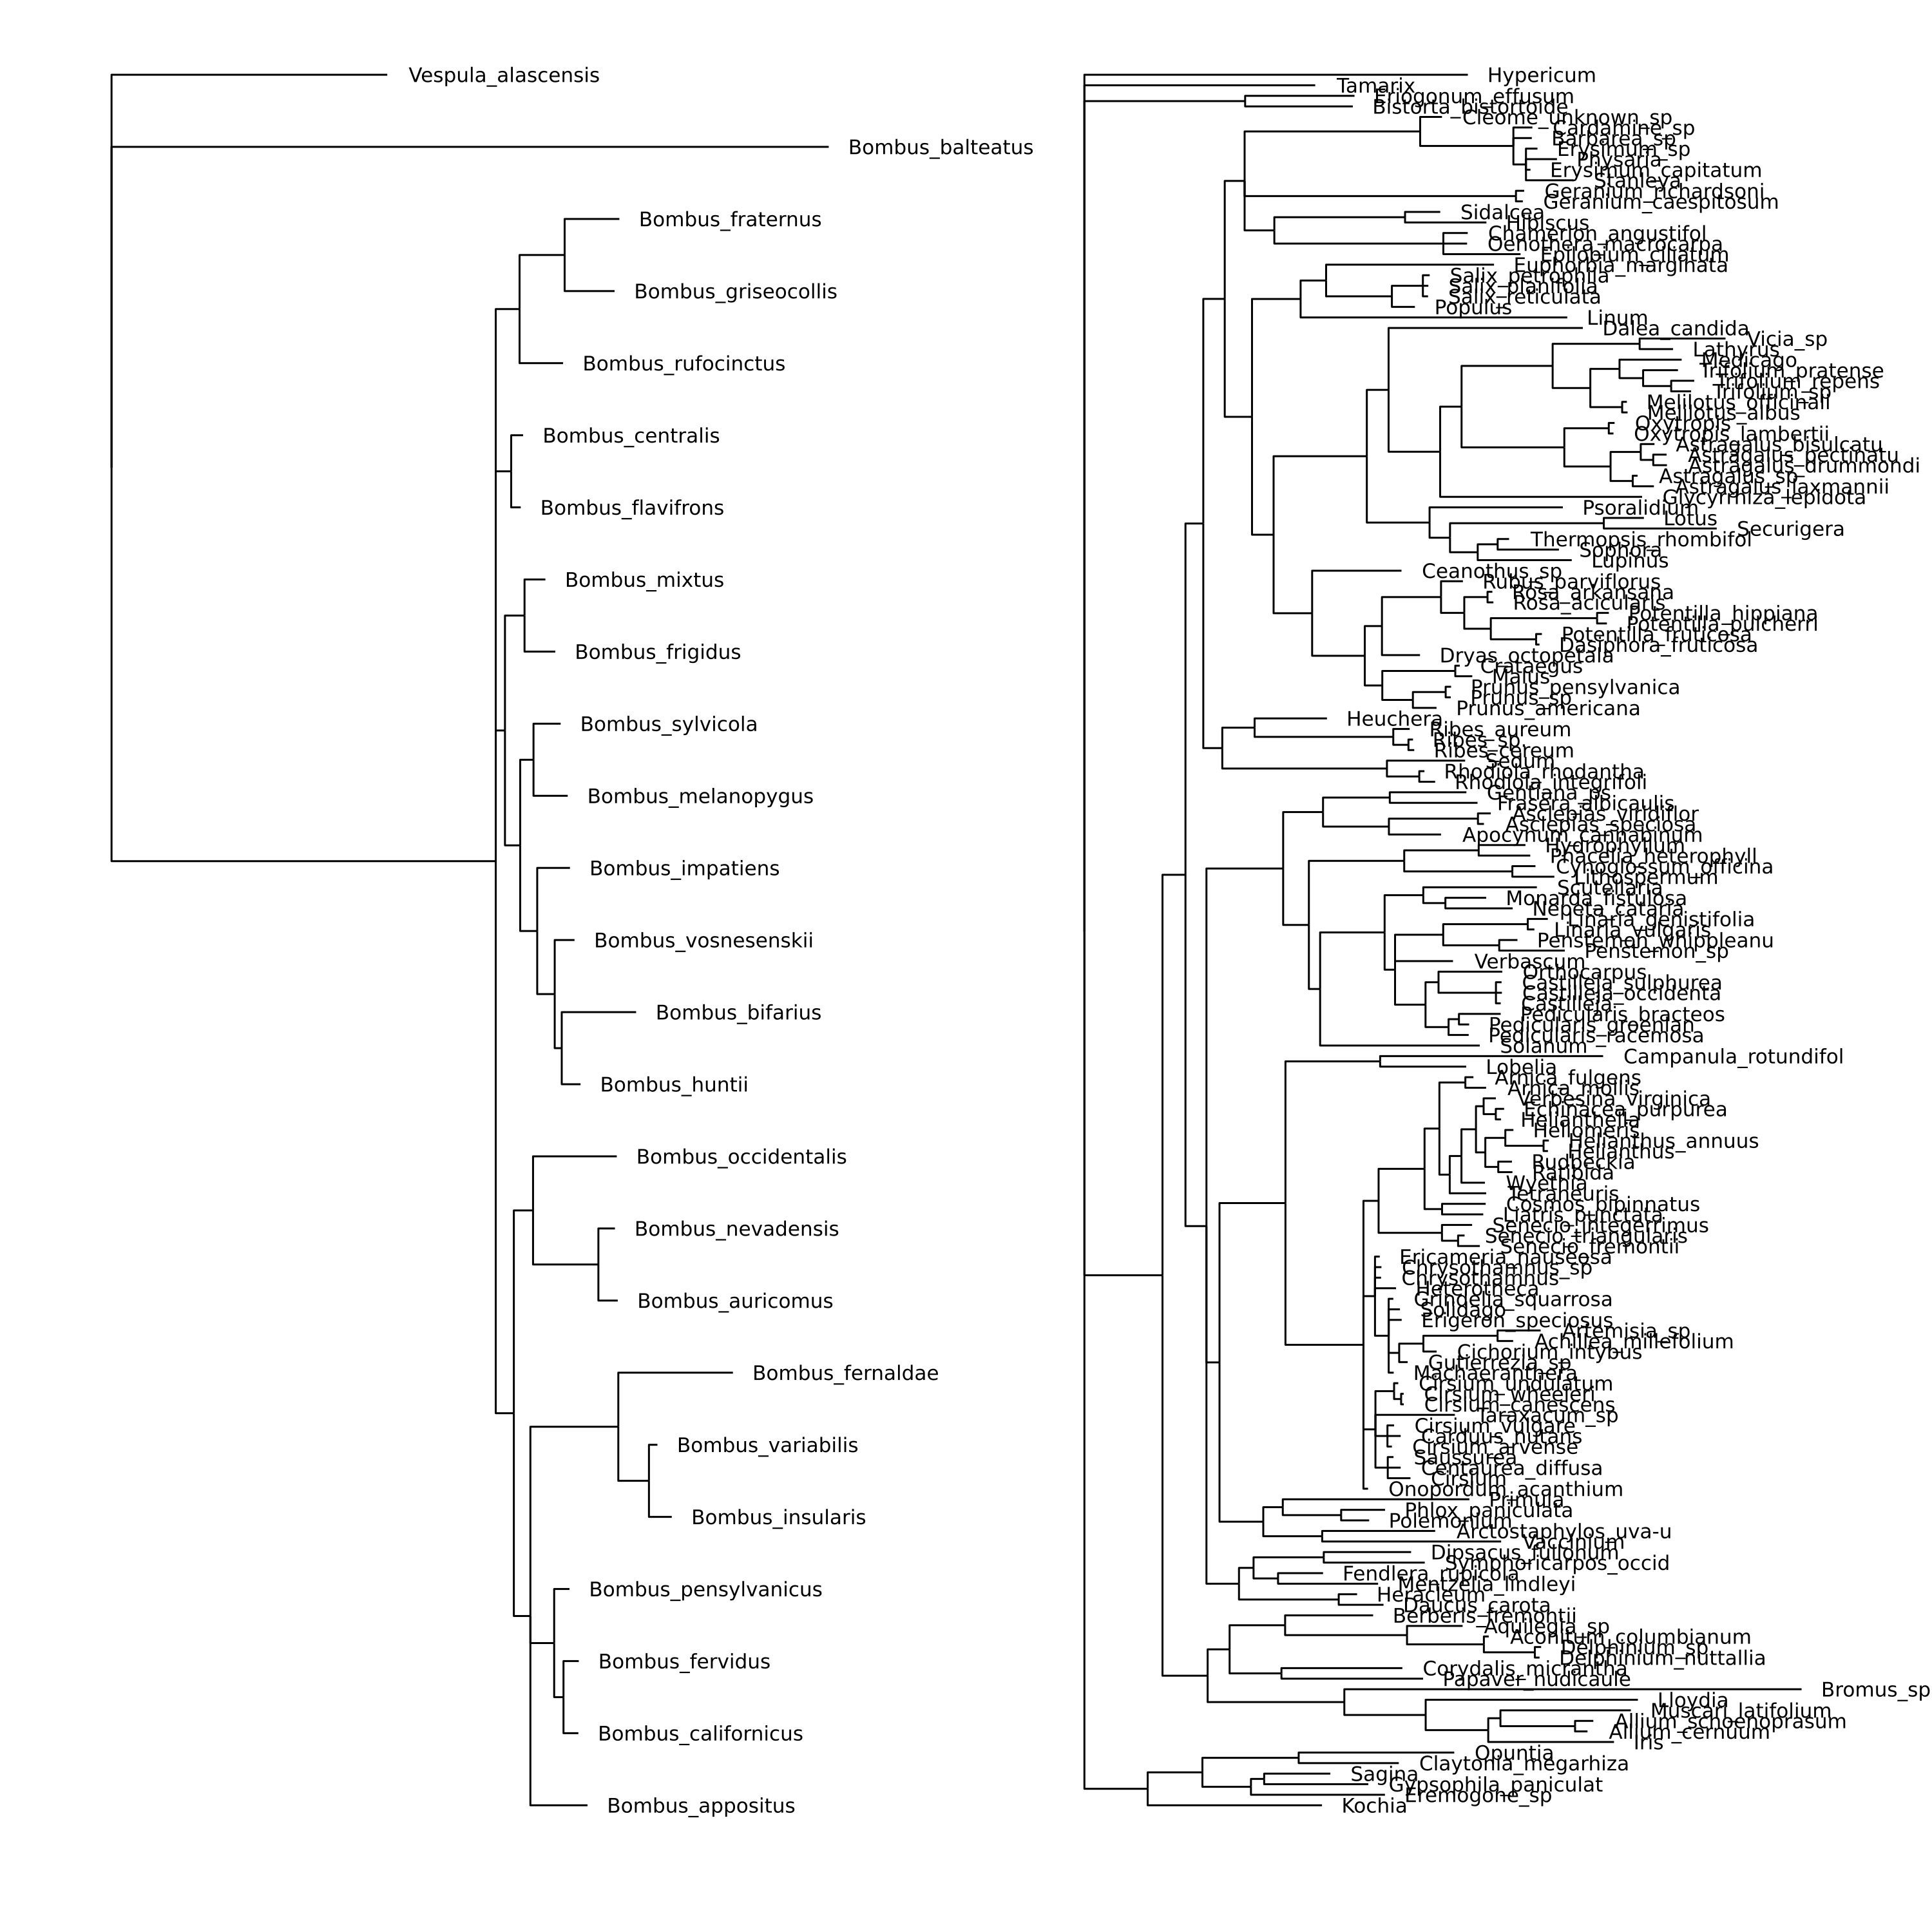
\includegraphics{./figures/trees.png}
\caption{trees}
\end{figure}

\hypertarget{references}{%
\section*{References}\label{references}}
\addcontentsline{toc}{section}{References}

\hypertarget{refs}{}
\begin{CSLReferences}{1}{0}
\leavevmode\hypertarget{ref-Bauer2015QuiRev}{}%
Bauer, P., Thorpe, A. \& Brunet, G. (2015). The quiet revolution of
numerical weather prediction. \emph{Nature}, 525, 47--56.

\leavevmode\hypertarget{ref-Beckage2011LimPre}{}%
Beckage, B., Gross, L.J. \& Kauffman, S. (2011). The limits to
prediction in ecological systems. \emph{Ecosphere}, 2, art125.

\leavevmode\hypertarget{ref-Chen2019RevCom}{}%
Chen, Y., Angulo, M.T. \& Liu, Y.-Y. (2019). Revealing Complex
Ecological Dynamics via Symbolic Regression. \emph{BioEssays}, 41,
1900069.

\leavevmode\hypertarget{ref-Dietze2017PreEco}{}%
Dietze, M.C. (2017). Prediction in ecology: A first-principles
framework. \emph{Ecological Applications}, 27, 2048--2060.

\leavevmode\hypertarget{ref-Hadfield2014TalTwo}{}%
Hadfield, J.D., Krasnov, B.R., Poulin, R. \& Nakagawa, S. (2014). A Tale
of Two Phylogenies: Comparative Analyses of Ecological Interactions.
\emph{The American Naturalist}, 183, 174--187.

\leavevmode\hypertarget{ref-Hanski2000MetCap}{}%
Hanski, I. \& Ovaskainen, O. (2000). The metapopulation capacity of a
fragmented landscape. \emph{Nature}, 404, 755--758.

\leavevmode\hypertarget{ref-Hubbell2001UniNeu}{}%
Hubbell, S.P. (2001). \emph{The unified neutral theory of biodiversity
and biogeography}. Monographs in population biology. Princeton
University Press, Princeton.

\leavevmode\hypertarget{ref-Makiola2020KeyQue}{}%
Makiola, A., Compson, Z.G., Baird, D.J., Barnes, M.A., Boerlijst, S.P.,
Bouchez, A., \emph{et al.} (2020). Key Questions for Next-Generation
Biomonitoring. \emph{Frontiers in Environmental Science}, 7.

\leavevmode\hypertarget{ref-Ovaskainen2002MetMod}{}%
Ovaskainen, O., Sato, K., Bascompte, J. \& Hanski, I. (2002).
Metapopulation Models for Extinction Threshold in Spatially Correlated
Landscapes. \emph{Journal of Theoretical Biology}, 215, 95--108.

\leavevmode\hypertarget{ref-Ovaskainen2002MetMod}{}%
Ovaskainen, O., Sato, K., Bascompte, J. \& Hanski, I. (2002).
Metapopulation Models for Extinction Threshold in Spatially Correlated
Landscapes. \emph{Journal of Theoretical Biology}, 215, 95--108.

\leavevmode\hypertarget{ref-Petchey2015EcoFor}{}%
Petchey, O.L., Pontarp, M., Massie, T.M., Kéfi, S., Ozgul, A.,
Weilenmann, M., \emph{et al.} (2015). The ecological forecast horizon,
and examples of its uses and determinants. \emph{Ecology Letters}, 18,
597--611.

\leavevmode\hypertarget{ref-Peterman2018ResRP}{}%
Peterman, W.E. (2018). ResistanceGA: An R package for the optimization
of resistance surfaces using genetic algorithms. \emph{Methods in
Ecology and Evolution}, 9, 1638--1647.

\leavevmode\hypertarget{ref-Thompson2000ResSol}{}%
Thompson, R.M. \& Townsend, C.R. (2000). Is resolution the solution?:
The effect of taxonomic resolution on the calculated properties of three
stream food webs. \emph{Freshwater Biology}, 44, 413--422.

\end{CSLReferences}

\end{document}
